\section{Análisis}

La ingeniería de requisitos proporciona el mecanismo apropiado para entender lo que dice el cliente, analizar las necesidades, evaluar la factibilidad, negociar una solución, especificar la solución sin ambigüedades, validar la especificación y administrar los requisitos a medida que se transforman en un sistema funcional\cite{pressman}.

\subsection{Casos de uso}
Para poder entender cómo los usuarios emplearán finalmente las funciones y características del software, se debe crear un conjunto de escenarios que identifiquen la naturaleza de los usos para el sistema que se va a construir. La descripción de la manera en la que se utilizará el sistema se la conoce como caso de uso.

\subsubsection{Actores del sistema}
Un actor es cualquier cosa que se comunica con el sistema o producto y que sea externo a este. 

\begin{table}[htpb]
\centering
\caption{Actores del sistema}
\label{tab_actores}
\begin{tabularx}{\textwidth}{|l|X|X|}
\hline
\multicolumn{1}{|c|}{Identificador} & \multicolumn{1}{c|}{Nombre} & \multicolumn{1}{c|}{Descripción}                                 \\ \hline
ACT-001                             & Usuario                     & Cualquier persona que acceda a nuestra plataforma web.           \\ \hline
ACT-002                             & Paciente                    & Cualquier persona que desee ser evaluada por nuestra aplicación. \\ \hline
ACT-003                             & Psicólogo                   & Cualquier persona que ejerza profesionalmente como psicólogo.    \\ \hline
ACT-004                             & Sistema                     & Encargado de ejecutar el algoritmo de emparejamiento.            \\ \hline
ACT-005                             & Administrador               & Persona encargada de gestionar los recursos de la aplicación.    \\ \hline
\end{tabularx}
\end{table}


\subsubsection{Especificación de casos de uso}
Para poder determinar y evaluar corréctamente cada caso de uso, tenemos una escala de la frecuencia de uso\ref{tab_frec_uso} y otra de la prioridad\ref{tab_prior}.

\begin{table}[htpb]
\centering
\caption{Frecuencias de uso}
\label{tab_frec_uso}
\begin{tabularx}{\textwidth}{|l|X|}
\hline
\multicolumn{2}{|c|}{Frecuencia de uso}                                                   \\ \hline
Ocasionalmente & Se utilizará en algunas ocasiones, no de forma habitual o por costumbre. \\ \hline
Puntualmente   & Se utilizará en raras ocasiones.                                         \\ \hline
Limitada       & Sólo podrá utilizarse en una única ocasión.                              \\ \hline
\end{tabularx}
\end{table}

\begin{table}[htpb]
\centering
\caption{Prioridades}
\label{tab_prior}
\begin{tabularx}{\textwidth}{|l|X|}
\hline
\multicolumn{2}{|c|}{Prioridad}                                                                          \\ \hline
Alta  & El caso de uso es imprescindible para el funcionamiento normal de la aplicación.                 \\ \hline
Media & El caso de uso aporta funcionalidad necesaria en el sistema pero no aporta un valor fundamental. \\ \hline
Baja  & El caso de uso aporta funcionalidades extra pero es totalmente prescindible.                     \\ \hline
\end{tabularx}
\end{table}

%
%CU-001
%

\begin{table}[htpb]
\centering
\caption{CU-001 Iniciar sesión}
%\label{my-label}
\begin{tabularx}{\textwidth}{|l|X|}
\hline
CU-001                            & Iniciar sesión                                                                                                                                                                                                                                   \\ \hline
Actor principal                   & Usuario                                                                                                                                                                                                                                          \\ \hline
Objetivo en contexto              & El actor desea acceder a una cuenta de usuario ya existente mediante sus claves de acceso.                                                                                                                                                       \\ \hline
Precondiciones                    & Las claves de usuario deben ser válidas.                                                                                                                                                                                                         \\ \hline
Disparador                        & El actor desea acceder a la plataforma para disfrutar de sus servicios.                                                                                                                                                                          \\ \hline
Escenario                         & \begin{tabular}{p{0.5cm} p{6cm}}1. & El actor accede a Emozio.\\ 2. & El actor introduce sus clavesde acceso.\\ 3. & El actor pulsa el botón de acceso.\\ 4. & El sistema muestra el perfil del actor donde podrá acceder al resto de servicios.\end{tabular} \\ \hline
Excepciones                       & \begin{tabular}{p{0.5cm} p{6cm}}1. & Las claves de usuario son incorrectas.\\ 2. & El actor no estaba registrado en la plataforma en el momento que se realizó el acceso.\end{tabular}                                                                    \\ \hline
Prioridad                         & Alta. El actor debe iniciar sesión en la aplicación para poder utilizar cualquiera de sus servicios.                                                                                                                                             \\ \hline
Disponibilidad                    & En el segundo incremento                                                                                                                                                                                                                         \\ \hline
Frecuencia de uso                 & Ocasionalmente                                                                                                                                                                                                                                   \\ \hline
Canal del actor                   & A través de un navegador con acceso a internet.                                                                                                                                                                                                  \\ \hline
Dependencias (con los requisitos) & \begin{tabular}[c]{@{}l@{}}RI-001\\ RI-003\\ RF-001\end{tabular}                                                                                                                                                                                 \\ \hline
\end{tabularx}
\end{table}

%
%CU-002
%

\begin{table}[]
\centering
\caption{CU-002 Registrarse}
%\label{my-label}
\begin{tabularx}{\textwidth}{|l|X|}
\hline
CU-002                            & Registrarse                                                                                                                                                                                                                                                                                                                                                                                                                    \\ \hline
Actor principal                   & Usuario                                                                                                                                                                                                                                                                                                                                                                                                                        \\ \hline
Objetivo en contexto              & El actor desea registrarse en la plataforma cediendo sus datos personales para poder acceder a los servicios de la plataforma.                                                                                                                                                                                                                                                                                                 \\ \hline
Precondiciones                    & Los datos introducidos en el formulario deben ser válidos.                                                                                                                                                                                                                                                                                                                                                                     \\ \hline
Disparador                        & El actor desea registrarse en la plataforma para disfrutar de sus servicios.                                                                                                                                                                                                                                                                                                                                                   \\ \hline
Escenario                         & \begin{tabular}{p{0.5cm} p{6cm}} 1. & El actor accede a Emozio. \\ 2. & El actor introduce sus datos en un formulario de registro.\\ 3. & El actor pulsa el botón de registro.\\ 4. & Se completa el registro.\\ 4.1. & Si es paciente, el sistema muestra el perfil del usuario donde podrá acceder al resto de servicios.\\ 4.2. & Si es psicólogo, sus datos son enviados por correo para que el administrador pueda validarlos.\end{tabular} \\ \hline
Excepciones                       & \begin{tabular}{p{0.5cm} p{6cm}}1. & Los datos introducidos en el formulario son incorrectos.\\ 2. & Ya existe el usuario dentro de la plataforma.\end{tabular}                                                                                                                                                                                                                                                                         \\ \hline
Prioridad                         & Alta. El actor debe estar registrado en la aplicación para poder utilizar cualquiera de sus servicios.                                                                                                                                                                                                                                                                                                                         \\ \hline
Disponibilidad                    & En el segundo incremento                                                                                                                                                                                                                                                                                                                                                                                                       \\ \hline
Frecuencia de uso                 & Limitada                                                                                                                                                                                                                                                                                                                                                                                                                       \\ \hline
Canal del actor                   & A través de un navegador con acceso a internet.                                                                                                                                                                                                                                                                                                                                                                                \\ \hline
Dependencias (con los requisitos) & \begin{tabular}[c]{@{}l@{}}RI-001\\ RI-003\\ RF-001\\ RF-002\end{tabular}                                                                                                                                                                                                                                                                                                                                                      \\ \hline
\end{tabularx}
\end{table}

%
%CU-003
%

\begin{table}[htpb]
\centering
\caption{CU-003 Realizar cuestionario}
%\label{my-label}
\begin{tabularx}{\textwidth}{|X|X|}
\hline
CU-003                            & Realizar cuestionario                                                                                                                                                                                                                                                                                                                                                                                                                                                                                                    \\ \hline
Actor principal                   & Paciente                                                                                                                                                                                                                                                                                                                                                                                                                                                                                                                 \\ \hline
Objetivo en contexto              & El paciente desea conocer qué profesional es el más adecuado para tratar su dolencia realizando el cuestionario de emparejamiento.                                                                                                                                                                                                                                                                                                                                                                                       \\ \hline
Precondiciones                    & El cuestionario debe estar cubierto.                                                                                                                                                                                                                                                                                                                                                                                                                                                                                     \\ \hline
Disparador                        & El paciente debe haber pulsado el botón de “hacer el cuestionario”.                                                                                                                                                                                                                                                                                                                                                                                                                                                      \\ \hline
Escenario                         & \begin{tabular} {p{0.5cm} p{5cm}} 1. & El  paciente accede a Emozio.\\ 2. & El paciente entra en su perfil de usuario ya sea por registro o acceso.\\  3. & El sistema le muestra su perfil de usuario.\\ 4. & El paciente pulsa el botón de hacer el cuestionario.\\ 5. & El sistema le muestra el formulario que debe cubrir.\\ 6. & El paciente cubre las respuestas del formulario.\\ 7. & El paciente pulsa el botón de conocerlos resultados.\\ 8. & El sistema le mostrará su perfil en el que se encuentran los resultados.\end{tabular} \\ \hline
Excepciones                       & Los datos introducidos en el formulario son incorrectos.                                                                                                                                                                                                                                                                                                                                                                                                                                                                 \\ \hline
Prioridad                         & Alta. Es la característica central de la plataforma.                                                                                                                                                                                                                                                                                                                                                                                                                                                                     \\ \hline
Disponibilidad                    & En el primer incremento                                                                                                                                                                                                                                                                                                                                                                                                                                                                                                  \\ \hline
Frecuencia de uso                 & Puntualmente                                                                                                                                                                                                                                                                                                                                                                                                                                                                                                             \\ \hline
Canal del actor                   & A través de un navegador con acceso a internet.                                                                                                                                                                                                                                                                                                                                                                                                                                                                          \\ \hline
Dependencias (con los requisitos) & \begin{tabular}[c]{@{}l@{}}RI-001\\ RI-002\\ RI-003\\ RF-001\\ RF-002\\  RF-005\end{tabular}                                                                                                                                                                                                                                                                                                                                                                                                                                       \\ \hline
\end{tabularx}
\end{table}

%
%CU-004
%

\begin{table}[htpb]
\centering
\caption{CU-004 Consultar resultados}
%\label{my-label}
\begin{tabularx}{\textwidth}{|X|X|}
\hline
CU-004                            & Consultar resultados                                                                                                                                                                                                                                                     \\ \hline
Actor principal                   & Paciente                                                                                                                                                                                                                                                                 \\ \hline
Objetivo en contexto              & El paciente desea consultar el resultado del cuestionario de asignación.                                                                                                                                                                                                 \\ \hline
Precondiciones                    & El cuestionario debe estar cubierto.                                                                                                                                                                                                                                     \\ \hline
Disparador                        & El paciente debe acceder a su perfil.                                                                                                                                                                                                                                    \\ \hline
Escenario                         & \begin{tabular}{p{0.5cm} p{5cm}} 1. & El paciente accede a Emozio. \\ 2. & El paciente entra en su perfil de usuario ya sea por registro o acceso.\\ 3. & El sistema le muestra su perfil de usuario donde se encuentran los resultados del cuestionario de asignación.\end{tabular} \\ \hline
Excepciones                       & El paciente no ha cubierto el test en ninguna ocasión.                                                                                                                                                                                                                   \\ \hline
Prioridad                         & Alta. Es la característica central de la plataforma.                                                                                                                                                                                                                     \\ \hline
Disponibilidad                    & En el primer incremento                                                                                                                                                                                                                                                  \\ \hline
Frecuencia de uso                 & Ocasionalmente                                                                                                                                                                                                                                                           \\ \hline
Canal del actor                   & A través de un navegador con acceso a internet.                                                                                                                                                                                                                          \\ \hline
Dependencias (con los requisitos) & \begin{tabular}[c]{@{}l@{}}RI-001\\ RI-003\\ RF-001\\ RF-002\\ RF-005\\ RF-006\end{tabular}                                                                                                                                                                                       \\ \hline
\end{tabularx}
\end{table}

%
%CU-005
%

\begin{table}[htpb]
\centering
\caption{CU-005 Contactar psicólogo}                                                                                                                                                                                                                                                                                                                                                                                                                                                                                                                                                                                                                                                                                                 
%\label{my-label}
\begin{tabularx}{\textwidth}{|X|X|}
\hline
CU-005                            & Contactar psicólogo                                                                                                                                                                                                                                                                                                                                                                                                                                                                                                                                                                                                                                                                                                        \\ \hline
Actor principal                   & Paciente                                                                                                                                                                                                                                                                                                                                                                                                                                                                                                                                                                                                                                                                                                                   \\ \hline
Objetivo en contexto              & El paciente desea ponerse en contacto con uno de los psicólogos que le han sido asignados.                                                                                                                                                                                                                                                                                                                                                                                                                                                                                                                                                                                                                                 \\ \hline
Precondiciones                    & \begin{tabular}{p{0.5cm} p{5cm}}1.  &  El cuestionario debe estar cubierto.\\ 2.  &  Las respuestas del cuestionario no dieron resultados imprecisos.\end{tabular}                                                                                                                                                                                                                                                                                                                                                                                                                                                                                                                                \\ \hline
Disparador                        & El paciente  accede a su perfil y se decide a contactar con el psicólogo.                                                                                                                                                                                                                                                                                                                                                                                                                                                                                                                                                                                                                                                  \\ \hline
Escenario                         & \begin{tabular}{p{0.5cm} p{5cm}}1.  &  El  paciente accede a Emozio.\\ 2.  &  El paciente entra en su perfil de usuario ya sea por registro o acceso.\\ 3.  &  El sistema le muestra su perfil de usuario donde se encuentran los resultados del cuestionario de asignación.\\ 4.  &  El paciente pulsa el botón de contacto del psicólogo en cuestión.\\ 5.  &  El sistema le muestra un formulario de contacto que debe cubrir.\\ 6.  &  El paciente cubre el formulario.\\ 7.  &  El paciente pulsa el botón de enviar.\\ 8.  &  El sistema muestra un mensaje con el estado de la operación.\end{tabular} \\ \hline
Excepciones                       & \begin{tabular}{p{0.5cm} p{5cm}}1.  &  El paciente no ha cubierto el test en ninguna ocasión.\\ 2.  &  El test dió un resultado impreciso para las respuestas dadas en el cuestionario.\end{tabular}                                                                                                                                                                                                                                                                                                                                                                                                                                                                                              \\ \hline
Prioridad                         & Moderada. Puede implementarse después de las funciones básicas.                                                                                                                                                                                                                                                                                                                                                                                                                                                                                                                                                                                                                                                            \\ \hline
Disponibilidad                    & En el tercer incremento                                                                                                                                                                                                                                                                                                                                                                                                                                                                                                                                                                                                                                                                                                    \\ \hline
Frecuencia de uso                 & Puntualmente                                                                                                                                                                                                                                                                                                                                                                                                                                                                                                                                                                                                                                                                                                               \\ \hline
Canal del actor                   & A través de un navegador con acceso a internet.                                                                                                                                                                                                                                                                                                                                                                                                                                                                                                                                                                                                                                                                            \\ \hline
Dependencias (con los requisitos) & \begin{tabular}[c]{@{}l@{}}RI-001\\ RI-003\\ RF-001\\ RF-002\\ RF-005\end{tabular}                                                                                                                                                                                                                                                                                                                                                                                                                                                                                                                                                                                             \\ \hline
\end{tabularx}
\end{table}

%
%CU-006
%

\begin{table}[htpb]
\centering
\caption{CU-006 Modificar información}                                                                                                                                                                                                                                                                                                                                                                                                                                                                           
%\label{my-label}
\begin{tabularx}{\textwidth}{|X|X|}
\hline
CU-006                            & Modificar información                                                                                                                                                                                                                                                                                                                                                                                                                                                                                \\ \hline
Actor principal                   & Usuario                                                                                                                                                                                                                                                                                                                                                                                                                                                                                              \\ \hline
Objetivo en contexto              & El usuario desea cambiar sus datos porque en ese instante su información de usuario es incorrecta.                                                                                                                                                                                                                                                                                                                                                                                                   \\ \hline
Precondiciones                    & El usuario tiene acceso a la plataforma.                                                                                                                                                                                                                                                                                                                                                                                                                                                             \\ \hline
Disparador                        & El usuario debe acceder a su página principal.                                                                                                                                                                                                                                                                                                                                                                                                                                                       \\ \hline
Escenario                         & \begin{tabular}{p{0.5cm} p{5cm}}1. & El usuario accede a Emozio.\\ 2. & El usuario entra en su página principal ya sea por registro o acceso.\\ 3. & El sistema le muestra su página principal.\\ 4. & El usuario pulsa el botón de modificación de datos.\\ 5. & El sistema le muestra un formulario con sus datos actuales.\\ 6. & El usuario cubre el formulario con los datos correctos.\\ 7. & El usuario pulsa el botón de enviar.\\ 8. & El sistema muestra un mensaje con el estado de la operación.\end{tabular} \\ \hline
Excepciones                       & El usuario cancela la operación en curso.                                                                                                                                                                                                                                                                                                                                                                                                                                                            \\ \hline
Prioridad                         & Moderada. Puede implementarse después de las funciones básicas.                                                                                                                                                                                                                                                                                                                                                                                                                                      \\ \hline
Disponibilidad                    & En el segundo incremento                                                                                                                                                                                                                                                                                                                                                                                                                                                                             \\ \hline
Frecuencia de uso                 & Puntualmente                                                                                                                                                                                                                                                                                                                                                                                                                                                                                         \\ \hline
Canal del actor                   & A través de un navegador con acceso a internet.                                                                                                                                                                                                                                                                                                                                                                                                                                                      \\ \hline
Dependencias (con los requisitos) & \begin{tabular}[c]{@{}l@{}}RI-001\\ RI-003\\ RF-001\\ RF-002\end{tabular}                                                                                                                                                                                                                                                                                                                                                                                                                            \\ \hline
\end{tabularx}
\end{table}

%
%CU-007
%

\begin{table}[htpb]
\centering
\caption{CU-007 Valorar psicólogo}
%\label{my-label}
\begin{tabularx}{\textwidth}{|X|X|}
\hline
CU-007                            & Valorar psicólogo                                                                                                                                                                                                                                                                                                                                                                                                                                                                                                                                                                                                                                                                  \\ \hline
Actor principal                   & Paciente                                                                                                                                                                                                                                                                                                                                                                                                                                                                                                                                                                                                                                                                           \\ \hline
Objetivo en contexto              & El paciente desea  valorar al psicólogo con el que se ha puesto en contacto.                                                                                                                                                                                                                                                                                                                                                                                                                                                                                                                                                                                                       \\ \hline
Precondiciones                    & El paciente se ha puesto en contacto previamente con el psicólogo en cuestión.                                                                                                                                                                                                                                                                                                                                                                                                                                                                                                                                                                                                     \\ \hline
Disparador                        & El paciente debe acceder al perfil del psicólogo.                                                                                                                                                                                                                                                                                                                                                                                                                                                                                                                                                                                                                                  \\ \hline
Escenario                         & \begin{tabular}{p{0.5cm} p{5cm}}1. & El  paciente accede a Emozio.\\ 2. & El paciente entra en su perfil de usuario ya sea por registro o acceso.\\ 3. & El sistema le muestra su perfil de usuario donde se encuentran los resultados del cuestionario de asignación.\\ 4. & El paciente pulsa el botón de mostrar más información del psicólogo.\\ 5. & El sistema le muestra el perfil del psicólogo seleccionado.\\ 6. & El paciente pulsa el botón de realizar valoración.\\ 7. & El sistema muestra un breve formulario que le permite valorar y escribir un mensaje.\\ 8. & El paciente pulsa el botón de enviar.\\ 9. & El sistema muestra un mensaje con el estado de la operación.\end{tabular} \\ \hline
Excepciones                       & \begin{tabular}{p{0.5cm} p{5cm}}1. & El paciente no se había puesto en contacto con el psicólogo previamente.\\ 2. & El paciente ya había dejado una valoración en el perfil del psicólogo.\end{tabular}                                                                                                                                                                                                                                                                                                                                                                                                                                                                                    \\ \hline
Prioridad                         & Moderada. Puede implementarse después de las funciones básicas.                                                                                                                                                                                                                                                                                                                                                                                                                                                                                                                                                                                                                    \\ \hline
Disponibilidad                    & En el tercer incremento                                                                                                                                                                                                                                                                                                                                                                                                                                                                                                                                                                                                                                                            \\ \hline
Frecuencia de uso                 & Puntualmente                                                                                                                                                                                                                                                                                                                                                                                                                                                                                                                                                                                                                                                                       \\ \hline
Canal del actor                   & A través de un navegador con acceso a internet.                                                                                                                                                                                                                                                                                                                                                                                                                                                                                                                                                                                                                                    \\ \hline
Dependencias (con los requisitos) & \begin{tabular}[c]{@{}l@{}}RI-001\\ RI-002\\ RF-001\\ RF-002\\ RF-005\\ RF-007\end{tabular}                                                                                                                                                                                                                                                                                                                                                                                                                                                                                                                                                                                                 \\ \hline
\end{tabularx}
\end{table}

%
%CU-008
%

\begin{table}[htpb]
\centering
\caption{CU-008 Filtrar resultados cuestionario}
%\label{my-label}
\begin{tabularx}{\textwidth}{|X|X|}
\hline
CU-008                            & Filtrar resultados cuestionario                                                                                                                                                                                                                                                                                                                                                                                                                                                               \\ \hline
Actor principal                   & Paciente                                                                                                                                                                                                                                                                                                                                                                                                                                                                                      \\ \hline
Objetivo en contexto              & El paciente desea filtrar su lista de psicólogos resultado en función de unos parámetros.                                                                                                                                                                                                                                                                                                                                                                                                     \\ \hline
Precondiciones                    & \begin{tabular}{p{0.5cm} p{5cm}}1. & El cuestionario debe estar cubierto.\\ 2. & Las respuestas del cuestionario no dieron resultados imprecisos.\end{tabular}                                                                                                                                                                                                                                                                                                                                         \\ \hline
Disparador                        & El paciente accede a su perfil y desea filtrar los resultados del cuestionario.                                                                                                                                                                                                                                                                                                                                                                                                               \\ \hline
Escenario                         & \begin{tabular}{p{0.5cm} p{5cm}}1. & El  paciente accede a Emozio.\\ 2. & El paciente entra en su perfil de usuario ya sea por registro o acceso.\\ 3. & El sistema le muestra su perfil de usuario donde se encuentran los resultados del cuestionario de asignación.\\ 4. & El paciente cubre el formulario de filtros que se muestra en la página.\\ 5. & El paciente pulsa el botón de enviar.\\ 6. & El sistema muestra el listado de resultados con los filtros que seleccionó el paciente.\end{tabular} \\ \hline
Excepciones                       & \begin{tabular}{p{0.5cm} p{5cm}}1. & El paciente no ha cubierto el test en ninguna ocasión.\\ 2. & El test dió un resultado impreciso para las respuestas dadas en el cuestionario.\end{tabular}                                                                                                                                                                                                                                                                                                       \\ \hline
Prioridad                         & Moderada. Puede implementarse después de las funciones básicas.                                                                                                                                                                                                                                                                                                                                                                                                                               \\ \hline
Disponibilidad                    & En el primer incremento                                                                                                                                                                                                                                                                                                                                                                                                                                                                       \\ \hline
Frecuencia de uso                 & Ocasionalmente                                                                                                                                                                                                                                                                                                                                                                                                                                                                                \\ \hline
Canal del actor                   & A través de un navegador con acceso a internet.                                                                                                                                                                                                                                                                                                                                                                                                                                               \\ \hline
Dependencias (con los requisitos) & \begin{tabular}[c]{@{}l@{}}RI-001\\ RI-003\\ RF-001\\ RF-002\\ RF-005\end{tabular}                                                                                                                                                                                                                                                                                                                                                                                                                     \\ \hline
\end{tabularx}
\end{table}

%
%CU-009
%

\begin{table}[htpb]
\centering
\caption{CU-009 Consultar perfil psicólogo}
%\label{my-label}
\begin{tabularx}{\textwidth}{|X|X|}
\hline
CU-009                            & Consultar perfil psicólogo                                                                                                                                                                                                                                                                                                                                                                                          \\ \hline
Actor principal                   & Paciente                                                                                                                                                                                                                                                                                                                                                                                                            \\ \hline
Objetivo en contexto              & El paciente desea consultar la información de perfil de uno de los psicólogos resultado.                                                                                                                                                                                                                                                                                                                            \\ \hline
Precondiciones                    & \begin{tabular}{p{0.5cm} p{5cm}}1. & El cuestionario debe estar cubierto.\\ 2. & Las respuestas del cuestionario no dieron resultados imprecisos.\end{tabular}                                                                                                                                                                                                                                                               \\ \hline
Disparador                        & El paciente debe acceder al perfil del psicólogo.                                                                                                                                                                                                                                                                                                                                                                   \\ \hline
Escenario                         & \begin{tabular}{p{0.5cm} p{5cm}}1. & El  paciente accede a Emozio.\\ 2. & El paciente entra en su perfil de usuario ya sea por registro o acceso.\\ 3. & El sistema le muestra su perfil de usuario donde se encuentran los resultados del cuestionario de asignación.\\ 4. & El paciente pulsa el botón de mostrar más información del psicólogo.\\ 5. & El sistema le muestra el perfil del psicólogo seleccionado.\end{tabular} \\ \hline
Excepciones                       & El paciente cancela la operación en curso.                                                                                                                                                                                                                                                                                                                                                                          \\ \hline
Prioridad                         & Moderada. Puede implementarse después de las funciones básicas.                                                                                                                                                                                                                                                                                                                                                     \\ \hline
Disponibilidad                    & En el primer incremento                                                                                                                                                                                                                                                                                                                                                                                             \\ \hline
Frecuencia de uso                 & Ocasionalmente                                                                                                                                                                                                                                                                                                                                                                                                      \\ \hline
Canal del actor                   & A través de un navegador con acceso a internet.                                                                                                                                                                                                                                                                                                                                                                     \\ \hline
Dependencias (con los requisitos) & \begin{tabular}[c]{@{}l@{}}RI-001\\ RI-003\\ RF-001\\ RF-002\\ RF-005\end{tabular}                                                                                                                                                                                                                                                                                                                                           \\ \hline
\end{tabularx}
\end{table}

%
%CU-010
%

\begin{table}[htpb]
\centering
\caption{CU-010 Darse de baja}                                                                                                                                                                                                                                                                                                                                                                                                                                                                                                                                                                                                  
%\label{my-label}
\begin{tabularx}{\textwidth}{|X|X|}
\hline
CU-010                            & Darse de baja                                                                                                                                                                                                                                                                                                                                                                                                                                                                                                                                                                                                   \\ \hline
Actor principal                   & Usuario                                                                                                                                                                                                                                                                                                                                                                                                                                                                                                                                                                                                         \\ \hline
Objetivo en contexto              & El usuario desea darse debaja en la aplicación.                                                                                                                                                                                                                                                                                                                                                                                                                                                                                                                                                                 \\ \hline
Precondiciones                    & El usuario tiene acceso a la plataforma.                                                                                                                                                                                                                                                                                                                                                                                                                                                                                                                                                                        \\ \hline
Disparador                        & El usuario debe acceder a su página principal.                                                                                                                                                                                                                                                                                                                                                                                                                                                                                                                                                                  \\ \hline
Escenario                         & \begin{tabular}{p{0.5cm} p{5cm}}1. & El usuario accede a Emozio.\\ 2. & El usuario entra en su página principal ya sea por registro o acceso.\\ 3. & El sistema le muestra su página principal.\\ 4. & El usuario pulsa el botón de modificación de datos.\\ 5. & El sistema le muestra un formulario con sus datos actuales, y un botón para darse de baja.\\ 6. & El usuario pulsa el botón de darse de baja.\\ 7. & El sistema muestra un pop-up pidiendo confirmación para ejecutar la operación.\\ 8. & El sistema elimina al usuario de la base de datos.\\ 9. & El sistema muestra al usuario la página de inicio.\end{tabular} \\ \hline
Excepciones                       & El usuario cancela la operación en curso.                                                                                                                                                                                                                                                                                                                                                                                                                                                                                                                                                                       \\ \hline
Prioridad                         & Moderada. Puede implementarse después de las funciones básicas.                                                                                                                                                                                                                                                                                                                                                                                                                                                                                                                                                 \\ \hline
Disponibilidad                    & En el segundo incremento                                                                                                                                                                                                                                                                                                                                                                                                                                                                                                                                                                                        \\ \hline
Frecuencia de uso                 & Limitada                                                                                                                                                                                                                                                                                                                                                                                                                                                                                                                                                                                                        \\ \hline
Canal del actor                   & A través de un navegador con acceso a internet.                                                                                                                                                                                                                                                                                                                                                                                                                                                                                                                                                                 \\ \hline
Dependencias (con los requisitos) & \begin{tabular}[c]{@{}l@{}}RI-001\\ RI-003\\ RF-001\\ RF-002\end{tabular}                                                                                                                                                                                                                                                                                                                                                                                                                                                                                                                                                \\ \hline
\end{tabularx}
\end{table}

%
%CU-011
%

\begin{table}[htpb]
\centering
\caption{CU-011 Consultar bandeja de entrada}
%\label{my-label}
\begin{tabularx}{\textwidth}{|X|X|}
\hline
CU-011                            & Consultar bandeja de entrada                                                                                                                                                                           \\ \hline
Actor principal                   & Psicólogo                                                                                                                                                                                              \\ \hline
Objetivo en contexto              & El psicólogo desea consultar las peticiones que le han llegado a su bandeja de entrada.                                                                                                                \\ \hline
Precondiciones                    & Estar registrado.                                                                                                                                                                                      \\ \hline
Disparador                        & El psicologo accede a su perfil y quiere consultar su bandeja de entrada.                                                                                                                              \\ \hline
Escenario                         & \begin{tabular}{p{0.5cm} p{5cm}}1. & El psicólogo accede a Emozio.\\ 2. & El psicólogo accede a su perfil de usuario.\\ 3. & El sistema le muestra los mensajes pendientes de su bandeja de entrada.\end{tabular} \\ \hline
Excepciones                       & -                                                                                                                                                                                                      \\ \hline
Prioridad                         & Moderada. Puede implementarse después de las funciones básicas.                                                                                                                                        \\ \hline
Disponibilidad                    & En el tercer incremento                                                                                                                                                                                \\ \hline
Frecuencia de uso                 & Ocasionalmente                                                                                                                                                                                         \\ \hline
Canal del actor                   & A través de un navegador con acceso a internet.                                                                                                                                                        \\ \hline
Dependencias (con los requisitos) & \begin{tabular}[c]{@{}l@{}}RI-001\\ RI-003\\ RF-001\\ RF-002\end{tabular}                                                                                                                                       \\ \hline
\end{tabularx}
\end{table}

%
%CU-012
%

\begin{table}[htpb]
\centering
\caption{CU-012 Responder solicitud paciente}
%\label{my-label}
\begin{tabularx}{\textwidth}{|X|X|}
\hline
CU-012                            & Responder solicitud paciente                                                                                                                                                                                                                                                                                                                                                \\ \hline
Actor principal                   & Psicólogo                                                                                                                                                                                                                                                                                                                                                                   \\ \hline
Objetivo en contexto              & El psicólogo desea responder a una de las peticiones que le han llegado a su bandeja de entrada.                                                                                                                                                                                                                                                                            \\ \hline
Precondiciones                    & Tener peticiones pendientes en la bandeja de entrada.                                                                                                                                                                                                                                                                                                                       \\ \hline
Disparador                        & El psicólogo accede a su perfil, consulta su bandeja de entrada y selecciona una de las peticiones.                                                                                                                                                                                                                                                                         \\ \hline
Escenario                         & \begin{tabular}{p{0.5cm} p{5cm}}1. & El psicólogo accede a Emozio.\\ 2. & El psicólogo accede a su perfil de usuario.\\ 3. & El sistema le muestra los mensajes pendientes de su bandeja de entrada.\\ 4. & El psicólogo selecciona una de las peticiones pendientes y la responde.\\ 5. & El sistema muestra un mensaje de éxito, y pasa la petición pendiente a respondida.\end{tabular} \\ \hline
Excepciones                       & -                                                                                                                                                                                                                                                                                                                                                                           \\ \hline
Prioridad                         & Moderada. Puede implementarse después de las funciones básicas.                                                                                                                                                                                                                                                                                                             \\ \hline
Disponibilidad                    & En el tercer incremento                                                                                                                                                                                                                                                                                                                                                     \\ \hline
Frecuencia de uso                 & Ocasionalmente                                                                                                                                                                                                                                                                                                                                                              \\ \hline
Canal del actor                   & A través de un navegador con acceso a internet.                                                                                                                                                                                                                                                                                                                             \\ \hline
Dependencias (con los requisitos) & \begin{tabular}[c]{@{}l@{}}RI-001\\ RI-003\\ RF-001\\ RF-002\end{tabular}                                                                                                                                                                                                                                                                                                            \\ \hline
\end{tabularx}
\end{table}

%
%CU-013
%

\begin{table}[htbp]
\centering
\caption{CU-013 Emparejamiento}                        
%\label{my-label}
\begin{tabularx}{\textwidth}{|X|X|}
\hline
CU-013                            & Emparejamiento                                                                                                             \\ \hline
Actor principal                   & Sistema                                                                                                                    \\ \hline
Objetivo en contexto              & El sistema realiza el emparejamiento paciente-psicólogo.                                                                   \\ \hline
Precondiciones                    & El paciente en cuestión se disponga a realizar el test.                                                                    \\ \hline
Disparador                        & El paciente selecciona “Hacer el test”.                                                                                    \\ \hline
Escenario                         & Cuando se envíen los resultados del test de un paciente, el sistema hará la correspondiente asignación paciente-psicólogo. \\ \hline
Excepciones                       & -                                                                                                                          \\ \hline
Prioridad                         & Alta. Es la característica central de la plataforma.                                                                       \\ \hline
Disponibilidad                    & En el primer incremento                                                                                                    \\ \hline
Frecuencia de uso                 & Ocasionalmente                                                                                                             \\ \hline
Canal del actor                   & A través de un navegador con acceso a internet.                                                                            \\ \hline
Dependencias (con los requisitos) & \begin{tabular}[c]{@{}l@{}}RI-001\\ RI-003\\ RF-001\\ RF-002\\  RF-005\end{tabular}                                                  \\ \hline
\end{tabularx}
\end{table}

%
%CU-014
%

\begin{table}[htpb]
\centering
\caption{CU-014 Dar alta a las preguntas}
%\label{my-label}
\begin{tabularx}{\textwidth}{|X|X|}
\hline
CU-014                            & Dar alta a las preguntas                                                                  \\ \hline
Actor principal                   & Administrador                                                                             \\ \hline
Objetivo en contexto              & El administrador dará de alta a las preguntas asociadas a las patologías.                 \\ \hline
Precondiciones                    & Tener nuevas preguntas para añadir al cuestionario.                                       \\ \hline
Disparador                        & Aparece una nueva patología o se modifican y/o actualizan las preguntas de una patología. \\ \hline
Escenario                         & El administrador añade las preguntas a la base de datos.                                  \\ \hline
Excepciones                       & -                                                                                         \\ \hline
Prioridad                         & Alta. Es la característica central de la plataforma.                                      \\ \hline
Disponibilidad                    & En el primer incremento                                                                   \\ \hline
Frecuencia de uso                 & Puntualmente                                                                              \\ \hline
Canal del actor                   & A través de una herramienta de gestión de bases de datos.                                 \\ \hline
Dependencias (con los requisitos) & RI-002                                                                                    \\ \hline
\end{tabularx}
\end{table}

%
%CU-015
%

\begin{table}[htpb]
\centering
\caption{CU-015 Añadir la publicidad}                          
%\label{my-label}
\begin{tabularx}{\textwidth}{|X|X|}
\hline
CU-015                            & Añadir la publicidad                                                                           \\ \hline
Actor principal                   & Administrador                                                                                  \\ \hline
Objetivo en contexto              & El administrador añadirá la publicidad necesaria a la aplicación en el momento que se precise. \\ \hline
Precondiciones                    & -                                                                                              \\ \hline
Disparador                        & El administrador quiere actualizar los contenidos publicitarios.                               \\ \hline
Escenario                         & El administrador añade las preguntas a la base de datos.                                       \\ \hline
Excepciones                       & -                                                                                              \\ \hline
Prioridad                         & Moderada. Puede implementarse después de las funciones básicas.                                \\ \hline
Disponibilidad                    & En el tercer incremento                                                                        \\ \hline
Frecuencia de uso                 & Puntualmente                                                                                   \\ \hline
Canal del actor                   & A través de una herramienta de edición de código.                                              \\ \hline
Dependencias (con los requisitos) & -                                                                                              \\ \hline
\end{tabularx}
\end{table}

\clearpage

%
%CU-016
%

\begin{table}[htpb]
\centering
\caption{CU-016 Dar alta psicólogos}                          
%\label{my-label}
\begin{tabularx}{\textwidth}{|X|X|}
\hline
CU-016                            & Dar alta psicólogos                                                                            \\ \hline
Actor principal                   & Administrador                                                                                  \\ \hline
Objetivo en contexto              & El administrador dará de alta a los psicólogos que hayan enviado el formulario de registro.    \\ \hline
Precondiciones                    & El psicólogo que se va a dar de alta, ha de haber cubierto el formulario de registro.          \\ \hline
Disparador                        & El administrador desea actualizar la colección de psicólogos de la base de datos.              \\ \hline
Escenario                         & El administrador añade la información del psicólogo a la base de datos.                        \\ \hline
Excepciones                       & -                                                                                              \\ \hline
Prioridad                         & Moderada. Puede implementarse después de las funciones básicas.                                \\ \hline
Disponibilidad                    & En el segundo incremento                                                                       \\ \hline
Frecuencia de uso                 & Puntualmente                                                                                   \\ \hline
Canal del actor                   & A través de un navegador con acceso a internet y una herramienta de gestión de bases de datos. \\ \hline
Dependencias (con los requisitos) & \begin{tabular}[c]{@{}l@{}}RI-003\\ RI-002\end{tabular}                                        \\ \hline
\end{tabularx}
\end{table}

\subsubsection{Diagrama de casos de uso}
Las relaciones entre los actores y los casos de uso viene dada por el diagrama de casos de uso\ref{fig:diag_casos_uso}.

%\begin{figure}[htbp] 
%    \centering
%    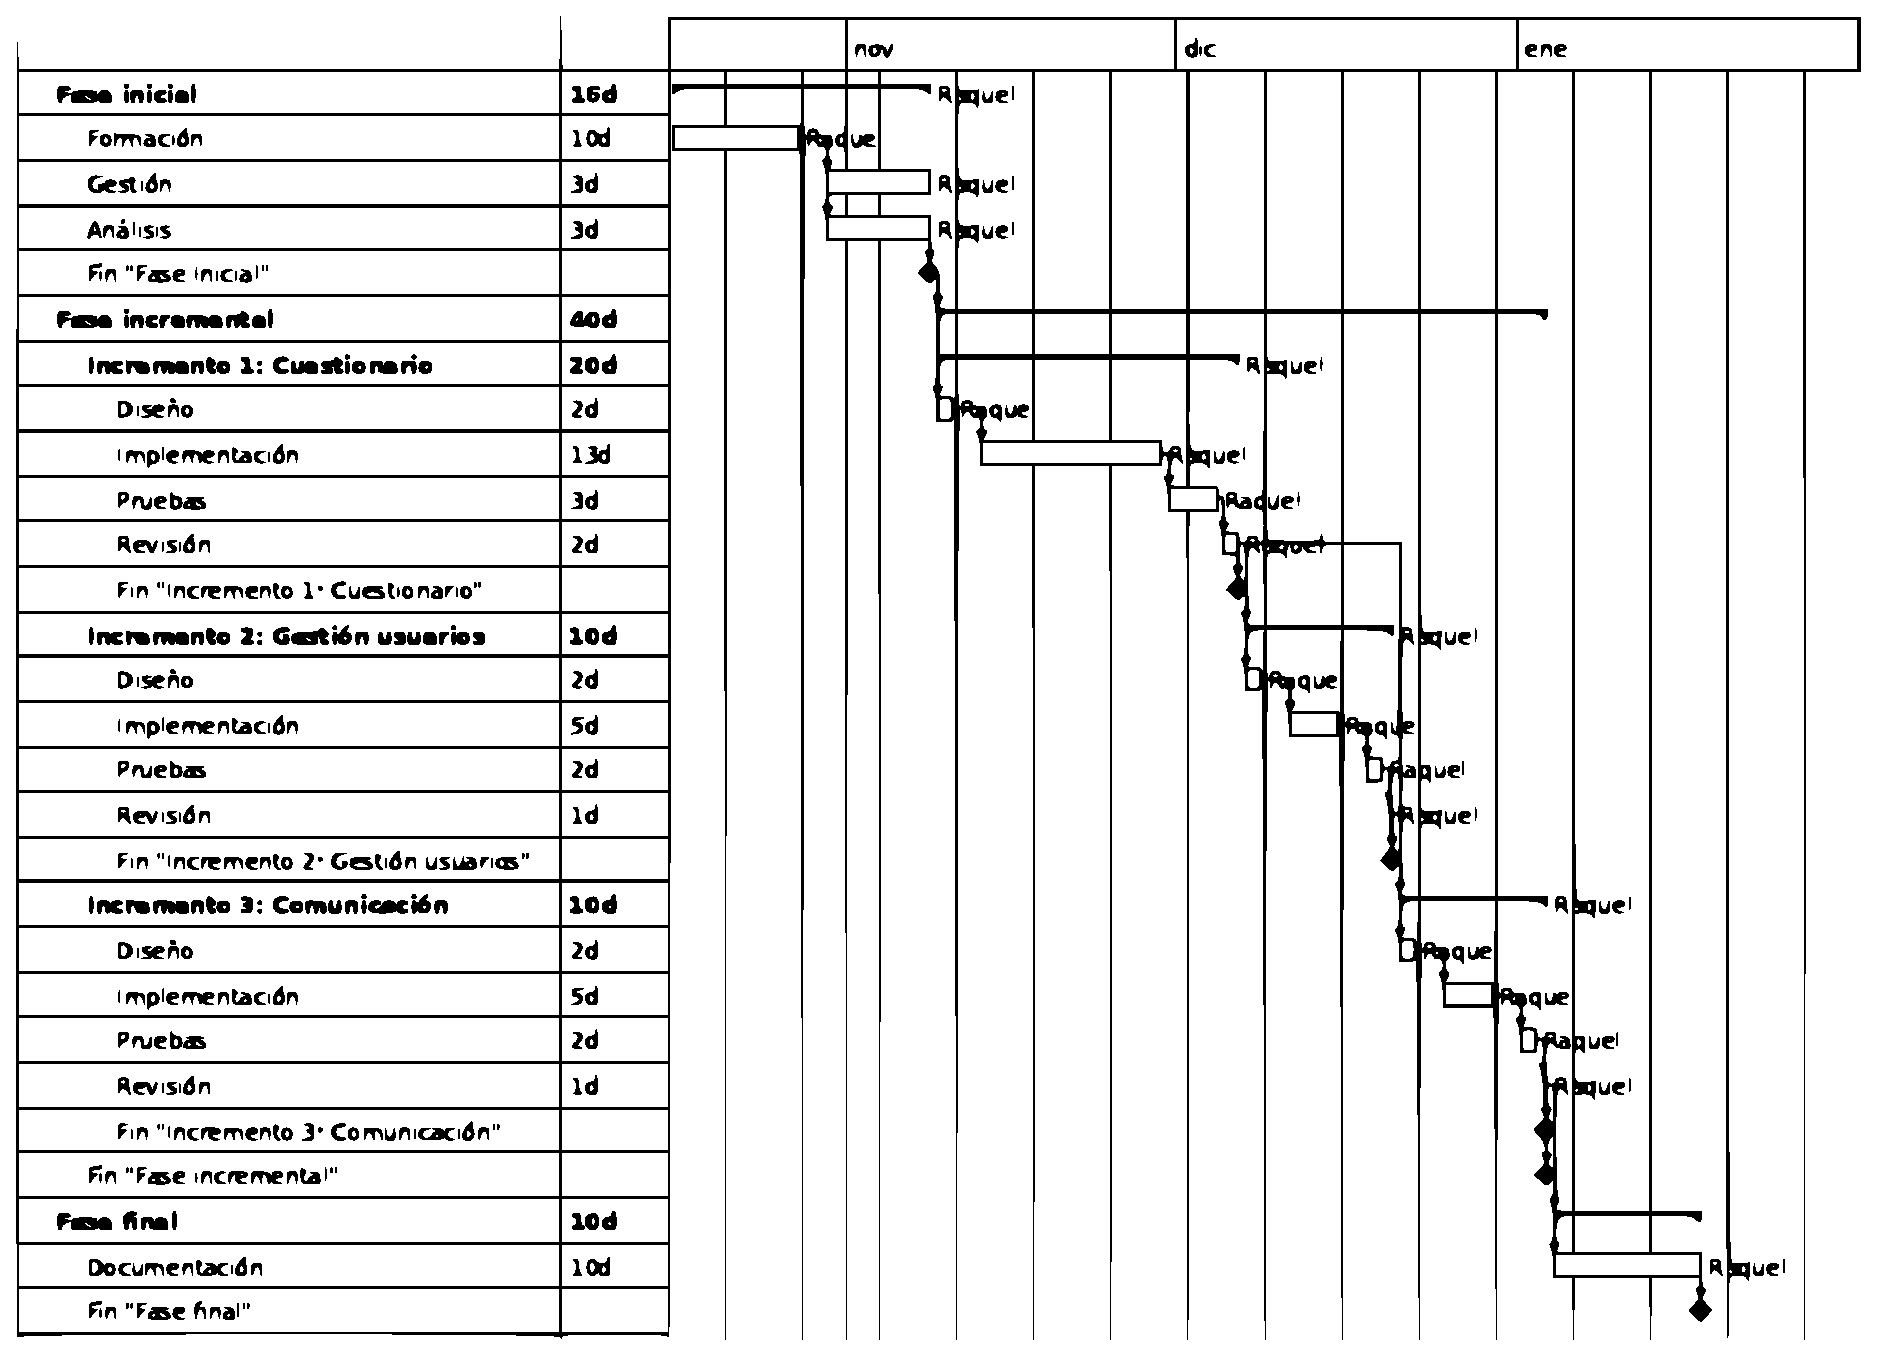
\includegraphics[width=1\textwidth]{figuras/gantt.eps}
%    \caption{Diagrama de casos de uso}
%    \label{fig:diag_casos_uso}
%\end{figure}	

\subsection{Modelado de datos}
Si los requisitos del software incluyen la necesidad de crear, ampliar o hacer interfaz con una base de datos, o si deben construirse y manipularse estructuras de datos complejas, se debe crear un modelo de datos como parte del modelado general de los requisitos.\cite{pressman}


Los modelos semánticos de datos son la definición de la forma lógica de los datos procesados por el sistema. \cite{sommerville}
